%!TEX TS-program = xelatex
%!TEX encoding = UTF-8 Unicode
\documentclass[a4paper]{report}
%\usepackage[date=short,backend=biber]{apa}
\usepackage[hidelinks]{hyperref}
\usepackage{cite}
\usepackage[dutch]{babel}
\usepackage[a4paper, left=1in, right=1in, top=1in, bottom=.8in]{geometry}
\usepackage[utf8]{inputenc}
\usepackage{fancyhdr}
\usepackage{titlesec}
\usepackage{geometry}
\usepackage{graphicx}
\usepackage{etoolbox}
\usepackage{listings}
\usepackage{xcolor}
\usepackage{nameref}
\usepackage{tcolorbox}
\usepackage{textcomp}
\usepackage{helvet}
\usepackage{enumitem}
\usepackage{tabularx}
\usepackage{pgf-pie}  
\usepackage{float}
\usepackage{pdfpages}
\usepackage{pgfplots}
\usepackage{multicol}

% Variables
\newcommand{\latestVersion}{2.1}

\newcommand{\styledhref}[2]{%
    \href{#1}{\textcolor{blue}{\underline{#2}}} % blue and underlined
}


% Double-page bibliography
\makeatletter
\renewenvironment{thebibliography}[1]
     {\renewcommand{\chapter}[2]{} % Removes the 'Chapter' heading
     \renewcommand{\addcontentsline}[3]{}
      \begin{multicols}{2}[]%
      \@mkboth{\MakeUppercase\refname}{\MakeUppercase\refname}%
      \list{\@biblabel{\@arabic\c@enumiv}}%
           {\settowidth\labelwidth{\@biblabel{#1}}%
            \leftmargin\labelwidth
            \advance\leftmargin\labelsep
            \@openbib@code
            \usecounter{enumiv}%
            \let\p@enumiv\@empty
            \renewcommand\theenumiv{\@arabic\c@enumiv}}%
      \sloppy
      \clubpenalty4000
      \@clubpenalty \clubpenalty
      \widowpenalty4000%
      \sfcode`\.\@m}
     {\def\@noitemerr
       {\@latex@warning{Empty `thebibliography' environment}}%
      \endlist\end{multicols}}
\makeatother
% Styling
\pagestyle{fancy}
\patchcmd{\chapter}{\thispagestyle{plain}}{\thispagestyle{fancy}}{}{}

\fancyhf{}
\fancyhead[L]{ Team Fairphone }
\fancyhead[R]{Verantwoordingsdocument }
\fancyfoot[R]{\thepage}

\titleformat{\chapter}[hang]
{\normalfont\huge\bfseries}{\thechapter.}{10pt}{\huge}
\titlespacing{\chapter}{0pt}{-30pt}{20pt}

\setlength{\parindent}{0.2em}

\textwidth=400pt
\geometry{
    left=25mm
}

\renewcommand{\contentsname}{Inhoudsopgave}



\definecolor{codegreen}{rgb}{0,0.6,0}
\definecolor{codegray}{rgb}{0.5,0.5,0.5}
\definecolor{codepurple}{rgb}{0.58,0,0.82}
\definecolor{backcolour}{rgb}{0.95,0.95,0.92}

\lstdefinestyle{mystyle}{
    backgroundcolor=\color{backcolour},   
    commentstyle=\color{codegreen},
    keywordstyle=\color{magenta},
    numberstyle=\tiny\color{codegray},
    stringstyle=\color{codepurple},
    basicstyle=\ttfamily\footnotesize,
    breakatwhitespace=false,         
    breaklines=true,                 
    captionpos=b,                    
    keepspaces=true,                 
    numbers=left,                    
    numbersep=5pt,                  
    showspaces=false,                
    showstringspaces=false,
    showtabs=false,                  
    tabsize=2
}

\lstset{style=mystyle}

% Commands
\newcommand{\teambox}{
  \begin{tcolorbox}[hbox, colback=blue!5!white,colframe=blue!75!black,
    left=.1mm, right=.1mm, top=.1mm, bottom=.1mm, fontupper=\scriptsize\sffamily]
    Team Keuze
  \end{tcolorbox}
}

\newcommand{\personalbox}{
  \begin{tcolorbox}[hbox, colback=green!5!white,colframe=green!75!black,
    left=.1mm, right=.1mm, top=.1mm, bottom=.1mm, fontupper=\scriptsize\sffamily]
    Persoonlijke Keuze
  \end{tcolorbox}
}
\newcommand{\teamchoice}[1]{
  \section[ #1 ]{#1~\mbox{\raisebox{-2.5pt}{\teambox}}}
}

\newcommand{\personalchoice}[1]{
  \section[ #1 ]{#1~\mbox{\raisebox{-2.5pt}{\personalbox}}}
}

\newcommand{\timestamp}[1]{
  \mbox{\scriptsize \textbf{Datum:} #1} \smallbreak
}

% Document
\begin{document}


% Title Page
\begin{titlepage}
  \begin{center}
      \vspace*{.6cm}
      \Huge
      \textbf{ Verantwoordingsdocument }\\
      \vspace{0.2cm}
      \small Vincent van Setten \\
      \small Zeilvis Helden (Team FairPhone)

      \normalsize


      \vspace{1cm}
      
\includegraphics[width=0.7\textwidth]{Images/zeilvis_helden.png}
      \vspace{1cm}
      \Large\\
      \textbf{In opdracht van}\\
      \large
      \textbf{Hogeschool Utrecht} \\
      
\includegraphics[width=0.2\textwidth]{Images/logouni.png}


      \vfill
    \end{center}
      \textbf{Student:} Vincent van Setten - 1734729 \\
      \textbf{Gilde:} TI Gilde, Groep D\\
      \textbf{Innovation Team:} Project FairPhone (499) \\
      \textbf{Document Versie:} \latestVersion \\
      \textbf{Datum:} \today \\
      \vspace{2cm}
\end{titlepage}



% ToC
\tableofcontents

\chapter{Versiebeheer}
\begin{table}[h]
    \centering
    \begin{tabular}{|c|c|c|p{5cm}|}
        \hline
        \textbf{Versie} & \textbf{Datum} & \textbf{Veranderingen}  \\
        \hline
        2.1   & 2023-11-15 & Peer reviews toegevoegd \\
        \hline
        2.0   & 2023-11-13 & Feedback verwerkt (zie \ref{verwerktefeedback1}) \\
        \hline
        1.9   & 2023-11-01 & Peer reviews toegevoegd \\
        \hline
        1.8   & 2023-10-31 & Feedback verwerkt: concrete keuzes kort apart vermelden, \\  & & versie nummers toegevoegd voor vergelijkingen \\
        \hline
        1.7   & 2023-10-11 & Peer reviews toegevoegd. Referenties ge-update. \\
        \hline
        1.6    & 2023-10-09 & Feedback verwerkt, OS keuze toegelicht, Container Software keuze toegevoegd \\
        \hline
        1.5    & 2023-09-26 & Ontvangen en gegeven peer reviews toegevoegd \\
        \hline
        1.4    & 2023-09-25 & Meer details en visuals toegevoegd \\
        \hline
        1.3    & 2023-09-24 & Referenties toegevoegd \\
        \hline
        1.2    & 2023-09-22 & Hoofdstuk docker toegevoegd en keuzes uitgebreid \\
        \hline
        1.1    & 2023-09-14 & Introductie en timestamps toegevoegd\\
        \hline
        1.0    & 2023-09-10 & Eerste Versie \\
        \hline
    \end{tabular}
    \caption{Versiebeheer}
\end{table}


\chapter{Introductie}
Dit document heeft als doel het beschrijven en beredeneren van belangrijke gemaakte keuzes binnen het Innovation project. 
Hiermee kunnen stakeholders, toekomstige teams en projectleiders eenvoudig zien welke keuzes zijn gemaakt en waarom deze zijn gemaakt.
Daarmee hoop ik meer inzicht te bieden in het verloop van het project en waarom voor bepaalde dingen zijn gekozen. 
\vspace{1.5cm}

\begingroup
\let\clearpage\relax
\chapter{Projectbeschrijving}
Vanuit de Hogeschool Utrecht heeft ons team de opdracht gekregen om verder te werken aan een port van SailfishOS voor de Fairphone 4.
SailfishOS is een open-source besturingssysteem gemaakt door een bedrijf, Jolla, uit Finland. Standaard ondersteund SailfishOS geen Fairphone 4.
Vorig jaar heeft een ander team al een minimale port werkend gekregen, namelijk de basis functies van een operating system. Er missen daarentegen nog een aantal belangrijke functies.
\par \smallskip
Ons hoofddoel is het toevoegen van ondersteuning van android applicaties, zonder afhankelijk te zijn van Google en haar Google Play Services\texttrademark. 
Onze opdrachtgever wil uitsluitend gebruik maken van open-source code en frameworks. De grootste reden hiervoor is omdat hij erg achter de open-source filosofie staat en dit graag wil voortzetten.
Naast het hoofddoel, gaan we ondersteuning toevoegen voor 4G door SailfishOS te updaten.
\endgroup

\chapter{Gemaakte Keuzes}
% \section{Persoonlijke Keuzes}
\personalchoice{IDE}
\subsubsection{Context}
\timestamp{2023-09-05}
Onze code gaan we schrijven met behulp van een IDE. Dit is een vrij arbitraire keuze, maar kan later in het project gevolgen hebben. 
Zo kan elke IDE zijn eigen methodes hebben voor het gebruik en delen van instellingen en linters. 
\par\smallskip
Er zijn een aantal grote IDE's die wij kunnen gebruiken voor dit project, welke wij hebben gekozen omdat we hier al eerder mee hebben gewerkt binnen de opleiding.
\begin{enumerate}
  \item \styledhref{https://visualstudio.microsoft.com/}{Visual Studio} - Dit is een grote IDE met een breed scala aan features.
  \item \styledhref{https://code.visualstudio.com/}{Visual Studio Code} - Dit is officieel geen echte IDE, maar kan helemaal samengesteld worden naar jouw eigen beeld.
  \item \styledhref{https://codelite.org/}{CodeLite} - Dit is een bekend open-source IDE, gemaakt voor meerdere programmeertalen.
\end{enumerate}

\subsubsection{Keuze}
\timestamp{2023-09-05}
Ik kies voor het gebruik van Visual Studio Code.


\subsubsection{Keuze Toelichting}
\timestamp{2023-09-05}
Voor de IDE heb ik gekozen voor Visual Studio Code. Officieel is het geen IDE, maar het wordt veelal wel gebruikt als een IDE. 
Door de vele extensies en aanpasbaarheid, kan deze editor volledig naar wens ingesteld worden. 
Het is een volledig persoonlijke keuze, maar iedereen in ons team heeft ook gekozen voor Visual Studio Code.
Dit kan in de toekomst werk schelen, doordat onze werkomgeving bij iedereen gelijk is.

\personalchoice{Laptop OS}
\subsubsection{Context}
\timestamp{2023-09-05}
Om aan Sailfish OS te kunnen werken in een ontwikkelomgeving moet er een keuze gemaakt worden op welk besturingssysteem de ontwikkelomgeving gaat draaien. 
Volgens de porting-guide van SailfishOS hebben we een 64-bit Linux kernel nodig om SailfishOS verder te ontwikkelen~\cite{sailfishportingguide}.
De mogelijkheden voor dit project zijn keuzes uit verschillende 64-bit Linux distributies. 

We hebben de volgende distributies vergeleken. De redenen voor de keuze van deze specifieke distributies staan hieronder verder toegelicht.
\begin{enumerate}
  \item \styledhref{https://archlinux.org/}{Arch Linux (2023.09.01)}
  \item \styledhref{https://ubuntu.com/}{Ubuntu (23.04)}
  \item \styledhref{https://www.debian.org/}{Debian (12.2.0)}
  \item \styledhref{https://manjaro.org/}{Manjaro (Plasma 2023.09.19)}
\end{enumerate}

\subsubsection{Keuze}
\timestamp{2023-09-05}
Ik kies voor Arch Linux als mijn besturingssysteem.

\subsubsection{Keuze Toelichting}
\timestamp{2023-09-05}
Als team hebben we gekozen om Ubuntu te gebruiken als besturingssysteem voor onze laptops. 
Dit hebben we gedaan om de volgende twee redenen.
\begin{enumerate}
  \item Het voorgaande team gebruikte ook Linux en gebruikte dit voor de ontwikkelomgeving~\cite{fairphonegithub}
  \item De root-omgeving van SailfishOS is gebaseerd op Ubuntu (20.04 LTS)~\cite{sailfishportingguide}.
\end{enumerate}

Persoonlijk heb ik er voor gekozen om af te wijken van de team keuze, omdat ik denk dat ik efficiënter kan werken met een ander besturingssysteem.
Mijn team ging hier mee akkoord. Ik zal de specifieke redenen hieronder toelichten.
\par\smallskip
Ik heb sterke voorkeuren aan mijn besturingssysteem. Zo heb ik graag een snel systeem met toegang tot de nieuwste packages, maar is gebruiksvriendelijkheid helemaal geen prioriteit.
Mijn prioriteiten heb ik voor het gemak getoond in het taartdiagram in figuur \ref{graph:spec_percentages}.
\begin{figure}[H]
  \centering
\begin{tikzpicture}

  \pie{30/Packages,
  25/Snelheid,
  25/Minimaliteit,
  15/Stabiliteit,
  5/Gebruiksvriendelijkheid}
  
\end{tikzpicture}
\caption{Belang van criteria}
\label{graph:spec_percentages}
\end{figure}

Zoals te zien in bovenstaand diagram, vind ik zelf packages het belangrijkst. 
Wat ik hiermee bedoel is de toegang tot programma's en daarbij ook nieuwe versies van programma's.
In Linux distributies worden programma's vooral gedownload vanaf package managers. Afhankelijk van de package manager kunnen programma's die hierop beschikbaar zijn behoorlijk achterlopen qua versie. 
\par\smallskip 
Met minimaliteit bedoel ik dat er weinig toegevoegd is aan het besturingssysteem. Dit heeft mijn persoonlijke voorkeur, omdat het hierdoor wat meer vrijheid biedt in de aanpasbaarheid en het over het algemeen wat sneller is. 
Ook gebruik ik op deze manier zo min mogelijk opslag, wat erg handig is in ons project.
\par\smallskip
Op basis van bovenstaande criteria ga ik de volgende distributies vergelijken. 
\begin{enumerate}
  \item Arch Linux (2023.09.01), omdat ik deze distributie al gebruik.
  \item Ubuntu (23.04), omdat deze gebruikt werd door het vorige team en wordt gebruikt door het team van SailfishOS~\cite{sailfishportingguide}.
  \item Debian (12.2.0), omdat dit een populaire distributie is, waar Ubuntu op is gebaseerd. Dit biedt een minimalistischer alternatief om te testen.
  \item Manjaro (Plasma 2023.09.19) omdat dit een gebruiksvriendelijke distributie is gebaseerd op Arch Linux. Deze wordt vaak aangeraden, naast Ubuntu.
\end{enumerate}

In de volgende tabel vergelijk ik de criteria. Op basis van deze criteria maak ik een toegelichte keuze\footnote{De scores in deze tabel zijn gebaseerd op subjectieve en anekdotische ervaringen, en algemene consensus binnen de Linux-gemeenschap. Zo is het, bijvoorbeeld, algemeen geaccepteerd in de Linux-gemeenschap dat een basisinstallatie van Arch Linux minimalistischer is dan een standaard Ubuntu-installatie.}.


\begin{table}[h]
  \centering
  \begin{tabular}{|l|c|c|c|c|c|}
    \hline
    \textbf{Besturingssysteem} & \textbf{Snelheid} & \textbf{Packages} & \textbf{Gebruiksgemak} & \textbf{Stabiliteit} & \textbf{Minimaliteit} \\
    \hline
    Arch Linux & ++ & ++ & - & + & + \\
    \hline
    Ubuntu & + & - & ++ & ++ & -- \\
    \hline
    Debian & ++ & - & + & + & ++ \\
    \hline
    Manjaro & + & ++ & ++ & ++ & - \\
    \hline
  \end{tabular}
  \caption{Criteria score per distributie}
  \label{tab:os_ratings}
\end{table}

\pagebreak 

\timestamp{2023-10-09}
Arch Linux is, wanneer simpel gehouden, sneller dan Ubuntu\cite{archvsubuntureddit}.
Dit komt doordat Arch Linux met minder packages wordt geleverd dan Ubuntu.
Ook is Arch Linux de kleinste ISO, wat een goede indicatie is voor minimaliteit. 
De groottes van de ISO bestanden zijn als volgt\footnote{Deze resultaten zijn van de laatste releases op 2023-09-10.}.
\begin{itemize}
  \item Arch Linux (2023.09.01): \styledhref{https://archlinux.org/download/}{804.3MB}.
  \item Ubuntu (23.04): \styledhref{https://ubuntu.com/download/desktop}{4.6GB}.
  \item Manjaro (Plasma 2023.09.19): \styledhref{https://download.manjaro.org/kde/23.0.2/manjaro-kde-23.0.2-230919-linux65.iso}{3.6GB}.
  \item Debian (12.2.0): \styledhref{https://www.debian.org/distrib/netinst\#smallcd}{628MB}.
\end{itemize}

\par\smallskip
\timestamp{2023-09-05}
In bovenstaande tabel is te zien dat de keuze toch ligt tussen Arch Linux en Manjaro.
Hiertussen is Arch Linux wat minimalistischer, maar is Manjaro normaal gesproken wat stabieler en gebruiksvriendelijker. 
\par\smallskip
Op basis van deze punten kies ik voor Arch Linux. 
Arch Linux biedt toegang tot de AUR. Dit is een package repository die wordt onderhouden door de Arch Linux community.
Dit stelt een breed scala aan packages tot mijn beschikking, waarvan vele direct worden gebouwd vanuit Github.
Hiermee heb ik toegang tot bijna elk programma dat beschikbaar is op Linux, met daarbij de laatste versie. 
Daarnaast is Arch Linux snel en erg stabiel wanneer er wordt gekozen voor de LTS kernel\cite{QuickTipsStableArch}.
Een LTS-kernel is een release van de Linux kernel met langdurige ondersteuning, die zich richt op stabiliteit en beveiliging door middel van uitgebreide tests en minder frequente updates.
Doordat deze meer getest wordt dan reguliere releases en minder vaak geüpdatet wordt, is er minder kans op bugs of vulnerabilities in de kernel\cite{enwiki:1177298994}.
\par\smallskip
Hoewel het verschil tussen Manjaro en Arch Linux erg klein is, heb ik meer ervaring met Arch Linux en kan deze beter aangepast worden naar mijn wensen. 
Dit zal me beter in staat stellen om efficient te werken gedurende het project.


\personalchoice{Opzetten ontwikkelsysteem}
\subsubsection{Context}
\timestamp{2023-09-05}
Voor het opzetten van de ontwikkelomgeving moest er een keuze gemaakt worden op welke manier Linux geïnstalleerd wordt op de laptop. 
De opties waren als volgt.
\begin{enumerate}
  \item Linux in een Virtual Machine (VM)
  \item Dual booten naast Windows
  \item Native runnen, dat wil zeggen "direct op de laptop, zonder tussenlagen"
\end{enumerate}

Dual booten naast Windows is exact hetzelfde als native qua performance, omdat het direct op de hardware runt. 
Het enige verschil ten opzichten van native is dat je minder opslag hebt voor de Linux installatie. Dit komt omdat er natuurlijk ook ruimte nodig is voor Windows en de applicaties en documenten op Windows. 
\par\smallskip
Native is sneller dan virtual machines. Dit komt door de overhead die wordt toegevoegd door de Hypervisor. 
Hoeveel overhead dit is, hangt sterk af van veel factoren. Dit zijn dingen zoals de cpu, andere systeemonderdelen, de instellingen van de virtual machine, etc. 
Daarnaast is in de meeste gevallen een deel van de CPU, RAM en schijf nodig voor de host-besturingssysteem.
Maar, dat native sneller is dan virtual machine wordt aangetoond in een 2014 onderzoek van IBM~\cite{felter2015updated}.
Hierin wordt de performance van kernel-level virtual machines vergeleken met Docker en native. 
Hieruit komt dat native sneller is dan zowel Docker als (K)VM's. 

\subsubsection{Keuze}
\timestamp{2023-09-05}
Ik kies er voor om Linux native te runnen.

\subsubsection{Keuze Toelichting}
\timestamp{2023-09-05}
Ik heb gekozen om het simpelweg native te runnen, omdat dit voor mij de meeste voordelen heeft.
Hoewel het snelheidsverschil tussen een VM en native niet verschrikkelijk is, voegt een VM wel onnodige overhead toe. 
Ik had al een native Linux installatie, dus ik had geen reden om over te stappen op een VM. 
Daarnaast heb ik ook geen Windows nodig, dus is dual booten ook onnodig. 
\par\smallskip
Native geeft mij dus het meeste opslag en de beste performance. 


\teamchoice{Communicatie}
\subsubsection{Context}
\timestamp{2023-09-05}
Binnen ons projectgroep zullen we veel moeten communiceren. Afspraken moeten gemaakt worden, bestanden moeten gedeeld worden en soms moeten we simpelweg vragen kunnen stellen.
Normaal zal communicatie eenvoudig zijn als we met elkaar aan tafel zitten, maar er zullen zich ook situaties voordoen waar we niet fysiek kunnen communiceren.
In dit geval zijn er duidelijke afspraken nodig voor hoe we communiceren.
\par \smallskip 
We hebben in totaal drie digitale omgevingen nodig.
\begin{enumerate}
  \item Een communicatiekanaal voor contact met de opdrachtgever.
  \item Een communicatiekanaal voor intern teamcontact.
  \item Een gedeelde plek voor bestandsopslag.
\end{enumerate}

De keuze van communicatiekanalen is gemaakt aan de hand van de volgende lijst aan communicatieplatforms, welke is opgesteld aan de hand van een aantal redenen.
De overweging elke optie binnen de lijst staat genoteerd aan de rechterzijde van tabel \ref{tab:comm_platforms}.
\begin{table}[H]
  \centering
  \begin{tabular}{|l|p{10cm}|}
    \hline
    \textbf{Platform} & \textbf{Overweging} \\
    \hline
    \styledhref{https://discord.com/}{Discord (Stable 241602 (86f279e))} & Discord werd overwogen vanwege de mogelijkheden georganiseerde kanalen binnen een groep. Ook had onze opdrachtgever hier een sterke voorkeur voor. \\
    \hline
    \styledhref{https://www.whatsapp.com/}{WhatsApp (2.23.20.79)} & WhatsApp was een optie vanwege de voorkeuren binnen het team. \\
    \hline
    \styledhref{https://www.microsoft.com/en-us/microsoft-teams/group-chat-software}{Microsoft Teams (23272.2708.2452.9689)} & Microsoft Teams stond op de lijst vanwege de integraties met andere Microsoft producten, zoals Word, en de voorkeur van onze Gilde meester. \\
    \hline
    \styledhref{https://slack.com/}{Slack (4.35.121)} & Slack werd overwogen vanwege het gebruik van deze software binnen een ander project en het hierbij erg rijk was een opties en organisatie \\
    \hline
    \styledhref{https://telegram.org/}{Telegram (4.10.3-3)} & Telegram was een optie vanwege de populariteit en de mogelijkheid om bestanden te delen. \\
    \hline
  \end{tabular}
  \caption{Overwegingen voor Communicatieplatforms}
  \label{tab:comm_platforms}
\end{table}
Overige communicatieplatforms zijn niet overwogen door een gebrek aan bekendheid binnen het team, of doordat deze opties essentiële features achter een betaling verschuilde.
We hebben binnen het team immers geen beschikbaar budget voor dit soort applicaties.
\par\smallskip
Voor de bestandsopslag hebben we twee grote spelers, namelijk Google Drive en OneDrive. 
Beide zijn goede opties met vergelijkbare features. De reden dat we hebben gekozen om deze twee methodes te vergelijken is de populariteit van deze opties.
Doordat deze opties zo populair zijn, hadden onze teamleden hier al accounts op en waren we al bekwaam in het gebruik van deze services.

\subsubsection{Keuze}
\timestamp{2023-09-05}
Wij kiezen voor het gebruik van:
\begin{enumerate}
  \item Discord (Met de opdrachtgever)
  \item Whatsapp (Binnen het team)
  \item OneDrive (Bestandsopslag)
\end{enumerate}

\subsubsection{Keuze Toelichting}
\timestamp{2023-09-05}
Om onze keuze te maken, hebben we voor- en nadelen tegenover elkaar gezet voor elk platform in de volgende tabel.
\begin{table}[H]
  \centering
  \begin{tabular}{|l|p{6cm}|p{6cm}|}
    \hline
    \textbf{Platform} & \textbf{Voordelen} & \textbf{Nadelen} \\
    \hline
    \styledhref{https://discord.com/}{Discord} & Georganiseerde kanalen, hoge aanpasbaarheid, opdrachtgever gebruikt het al, bekendheid binnen het team. & Minder organisatie features dan alternatieven. \\
    \hline
    \styledhref{https://www.whatsapp.com/}{WhatsApp} & Snel en eenvoudig, geen nieuwe installaties nodig binnen team. Sterke teamvoorkeur. & Beperkte bestandsgrootte voor delen, afhankelijk van telefoonnummer. Weinig organisatie-tools. \\
    \hline
    \styledhref{https://www.microsoft.com/en-us/microsoft-teams/group-chat-software}{Microsoft Teams} & Goede integratie met Microsoft-producten, ondersteund door de Hogeschool. & Werkt niet goed op bepaalde Linux distributies. Niet open-source. Betaalde functies. \\
    \hline
    \styledhref{https://slack.com/}{Slack} & Rijk aan functies, goede organisatie van kanalen, integraties met andere tools. & Betaalde functies voor volledige toegang, kan ingewikkeld zijn om op te zetten. \\
    \hline
    \styledhref{https://telegram.org/}{Telegram} & Snel, mogelijkheid om grote bestanden te delen, cloud-gebaseerde opslag. & Minder populair in zakelijke context, weinig bekendheid binnen team \\
    \hline
  \end{tabular}
  \caption{Voordelen en Nadelen van Communicatieplatforms}
  \label{tab:comm_pros_cons}
\end{table}

Op basis van bovenstaande voor- en nadelen hebben we als team de volgende keuzes gemaakt als communicatiemiddelen.
\par\smallskip
Om contact te houden met de opdrachtgever hebben we gekozen voor een Discord server.
We hebben hiervoor gekozen, omdat de opdrachtgever Discord gebruikt en elk teamlid hier al actief gebruik van maakte.
\par \smallskip 
Voor intern teamcontact gebruiken we een Whatsapp groep. Dit vond het team unaniem de beste optie. Hiermee kunnen we snel met elkaar in contact komen en hoeven we geen nieuwe apps te installeren. 
\par \smallskip
Voor bestandsopslag gebruiken we OneDrive. Vanuit de Hogeschool Utrecht krijgen we allemaal standaard een OneDrive omgeving.
Hier hebben we meer dan voldoende opslag voor bestanden. OneDrive integreert ook gemakkelijk met Microsoft Word. 
Dat was voor ons reden genoeg om te kiezen voor OneDrive boven Google Drive.

\teamchoice{Wel of niet gebruik maken van Container Software}
\label{sec:dockerchoice}
\subsubsection{Context}
\timestamp{2023-09-20}
De huidige build environment wordt opgezet aan de hand van een installation guide~\cite{fairphonegithub}.
Daarnaast is er een installatiescript aanwezig.
Deze zouden moeten werken, maar hebben we dit tot nu toe nergens gemakkelijk werkend gekregen.
Tijdens het debuggen gaat het steeds fout op verschillende punten. 
We vermoeden dat dit komt door overblijvende build files die naar allemaal onbekende plekken in ons systeem worden geschreven, gebaseerd op eerdere ervaringen in eerdere projecten.
Door gebruik te maken van Container Software kunnen we dit voorkomen, omdat hiermee elke keer dezelfde stappen automatisch uitgevoerd kunnen worden vanaf het begin.

\subsubsection{Keuze}
\timestamp{2023-09-20}
Wij kiezen voor het wel gebruiken van Container Software.

\subsubsection{Keuze Toelichting}
\timestamp{2023-09-20}
Met oog op overdraagbaarheid denken wij als team dat het een goede keuze is om een Container environment op te gaan zetten. 
Hiermee zou de build environment eenvoudig overdraagbaar zijn en zou het gemakkelijk werken op in principe elk systeem, zonder dat er build files overblijven na een compilatie.
Dit zou ook tijd kunnen gaan schelen tijdens het debuggen~\cite{AffinityBridgeDockerProsCons}. 
\par\smallskip
Deze keuze staat tegenover een keuze gemaakt door een voorgaand ontwikkelingsteam binnen het Fairphone project. 
Het vorige team koos er voor om niet verder te gaan met container, omdat dit vrij lastig bleek en er tegen problemen werd gelopen. 
Zo liepen zij onder andere tegen problemen aan met permissions.
Wij geloven dat het waardevol is om toch hiermee verder te gaan, omdat dit de overdraagbaarheid enorm vergroot. Wij denken dat deze problemen niet onoverkomelijk zijn.
Hoewel het ons nu meer tijd zal kosten om dit op te zetten, zal dit een potentieel toekomstig ontwikkelingsteam enorm veel tijd schelen.
Wij hebben tijdens scrum poker 20 manuren geschat voor de opzet van container. Hoewel dat waarschijnlijk meer is dan het zou kosten om de build environment nu op te lossen, schatten wij dat de build environment meer problemen zal veroorzaken op een later stadium. 
Zo is het vorige team daar meerdere sprints mee bezig geweest en leek het steeds op andere punten fout te gaan.

\par\smallskip
De laatste reden voor het opzetten van de container omgeving, is omdat de opdrachtgever hier een sterke voorkeur voor had. Door het opzetten van een container omgeving, zal een toekomstig team geen weken meer bezig zijn om de build environment op te zetten. In plaats daarvan zal het minder dan een dagdeel moeten duren, namelijk het installeren van de container software en het runnen van de container.

\personalchoice{Container Software}
\subsubsection{Context}
\timestamp{2023-10-09}
Zoals toegelicht in hoofdstuk \ref{sec:dockerchoice}, gaan we gebruik maken van software om de build environment deels te virtualiseren, zodat het eenvoudig werkt op elk systeem.
Binnen ons team was Docker het meest bekend. We liepen tegen een aantal problemen aan met Docker op sommige systemen. 
Hierdoor besloten we te kijken naar alternatieven. Deze hebben we gevonden. De alternatieven maken allemaal gebruik van het \styledhref{https://opencontainers.org/}{\textit{Open Container Initiative}}.
Dit betekent dat we een Dockerfile ook zou moeten werken voor alternatieven die hiervan gebruik maken.
\par\smallskip
Docker had op een aantal computers errors, die zich op andere computers zich niet voordeden. 
Omdat Docker gebaseerd is op het OpenContainer Initiative, wilden we kijken of het misschien wel werkte met een alternatief.
Volgens \styledhref{https://alternativeto.net/software/docker/}{AlternativeTo} is Podman het populairste alternatief.
\par\smallskip
Bij het testen van onze Docker image met Podman, bleken deze errors zich niet voor te doen.
\par\smallskip 
Later besloten we de Docker image anders te structureren, wat ook de error met Docker liet verdwijnen op alle systemen. 
Toch hebben we de keuze geboden aan elk teamlid om zelf te kiezen voor hun container software.

\subsubsection{Keuze}
\timestamp{2023-10-09}
Ik kies voor het gebruik van Podman.

\subsubsection{Keuze Toelichting}
\timestamp{2023-10-09}
Hoewel zowel Docker als Podman nu werken op mijn systeem, kies ik persoonlijk voor het gebruik van Podman.
De grootste reden hiervoor is dat Podman werkt met rootless containers. Docker werkt door middel van een enkele Daemon\footnote{\styledhref{https://www.techtarget.com/whatis/definition/daemon}{Een service die op de achtergrond draait} } die runt met root privileges. 
Alle Docker instanties praten vervolgens met deze enkele Daemon, wat vervolgens de taken uitvoert. Doordat de Daemon root access heeft, kan dit security risico's met zich meebrengen als deze niet goed gebruikt wordt\cite{dockerdaemonrisks}.
Podman is wel langzamer dan Docker, maar deze verschillen zijn praktisch gezien vrij insignificant\cite{dockerperformance}.


\chapter{Bibliografie}
% \nocite{*} % This includes all entries from the .bib file, even if they're not cited in the document
\begingroup

\bibliographystyle{IEEEtran}
\bibliography{IEEEabrv,bronnen}
\endgroup

\chapter{Bijlagen}
\section{Gegeven Peer Reviews}
\subsection{Iteratie 1}
\subsubsection{Remy de Bruijn}
\noindent
\begin{minipage}{\textwidth}
  \centering
  \fbox{
  
\includegraphics[page=4,scale=0.7]{Appendices/Iteratie 1/PR Remy.pdf}}
\end{minipage}


\includepdf[pages={5},scale=0.7,frame,pagecommand={}]{Appendices/Iteratie 1/PR Remy.pdf}
\subsubsection{Joris Maas}
\begin{minipage}{\textwidth}
  \centering
  \fbox{
  
\includegraphics[page=4,scale=0.7]{Appendices/Iteratie 1/PR Joris.pdf}}
\end{minipage}


\includepdf[pages={5},scale=0.7,frame,pagecommand={}]{Appendices/Iteratie 1/PR Joris.pdf}


\subsection{Iteratie 2}
\subsubsection{Kyrill Westdorp}
\noindent
\begin{minipage}{\textwidth}
  \centering
  \fbox{
  
\includegraphics[page=4,scale=0.7]{Appendices/Iteratie 2/PR Kyrill.pdf}}
\end{minipage}


\includepdf[pages={5},scale=0.7,frame,pagecommand={}]{Appendices/Iteratie 2/PR Kyrill.pdf}
\subsubsection{Jasper Middendorp}
\begin{minipage}{\textwidth}
  \centering
  \fbox{
  
\includegraphics[page=4,scale=0.7]{Appendices/Iteratie 2/PR Jasper.pdf}}
\end{minipage}


\includepdf[pages={5},scale=0.7,frame,pagecommand={}]{Appendices/Iteratie 2/PR Jasper.pdf}


\subsection{Iteratie 3}
\subsubsection{Joris Maas}
\noindent
\begin{minipage}{\textwidth}
  \centering
  \fbox{
  
\includegraphics[page=3,scale=0.7]{Appendices/Iteratie 3/PR Joris.pdf}}
\end{minipage}

\subsubsection{Remy de Bruijn}
\noindent
\begin{minipage}{\textwidth}
  \centering
  \fbox{
  
\includegraphics[page=3,scale=0.7]{Appendices/Iteratie 3/PR Remy.pdf}}
\end{minipage}

\subsection{Iteratie 4}
\subsubsection{Jasper Middendorp}
\noindent
\begin{minipage}{\textwidth}
  \centering
  \fbox{
  
\includegraphics[page=3,scale=0.7]{Appendices/Iteratie 4/PR Jasper.pdf}}
\end{minipage}

\subsubsection{Kyrill Westdorp}
\noindent
\begin{minipage}{\textwidth}
  \centering
  \fbox{
  
\includegraphics[page=3,scale=0.7]{Appendices/Iteratie 4/PR Kyrill.pdf}}
\end{minipage}

\clearpage

\section{Ontvangen Peer Reviews}
\subsection{Iteratie 1}
\subsubsection{Kyrill Westdorp}
Van Kyrill heb ik de volgende tips gekregen.
\begin{enumerate}
  \item Aan het eind van je inleiding staat “Daarmee hopen wij meer inzicht te bieden in het verloop van het project en waarom voor bepaalde dingen zijn gekozen.” Ik zou er niet neerzetten hopen wij meer maar hoop ik meer inzicht te bieden in het verloop van het project en waarom voor bepaalde dingen is gekozen. Dit omdat als je wij gaat zeggen leg je de verantwoordelijkheid van dit document ook bij je groepsleden neer en dat klopt voor mijn gevoel niet omdat dit een persoonlijk document is (behalve de teamkeuzes dan).
  \item Bij je Projectbeschrijving zou ik graag wat meer uitleg willen waarom je niet afhankelijk wil zijn van Google en haar Play Services.
\end{enumerate}
En de volgende tops:
\begin{enumerate}
  \item Je uitleg over de keuze welk besturingssysteem jullie als team hebben gekozen en waarom je ervan afwijkt.
  \item Je maakt heel duidelijk waarom je afwijkt van de teamkeuze en beargumenteert die goed.
  \item De taartdiagram en de tabel geven extra duidelijkheid en zijn makkelijk af te lezen.
  \item Voor elke keuze geef je netjes andere opties weer en je legt duidelijk uit wat je keuze is uit die opties en waarom.
\end{enumerate}

De feedback van Kyrill is duidelijk en concreet. Hij licht toe waarom bepaalde dingen verbeterd kunnen worden, in plaats van alleen te vertellen wat er beter kan. 
Aan de hand van de feedback ga ik de volgende dingen verbeteren voor de volgende iteratie:
\begin{enumerate}
  \item De inleiding aanpassen, zodat er niet 'wij' staat. Het is een persoonlijk document, dus het is inderdaad raar dat ik daar 'wij' gebruik. 
  \item In de projectbeschrijving ga ik toelichten waarom we niet afhankelijk willen zijn van Google en haar play services, omdat dit een belangrijk standpunt is dat we hebben ingenomen. Dit maakt het duidelijker waarom ik voor bepaalde keuzes zijn gegaan in het document.
\end{enumerate}

\subsubsection{Jasper Middendorp}
Van Jasper heb ik de volgende tips gekregen.
\begin{enumerate}
  \item In de zin “bij het volgende taartdiagram” in Laptop OS keuze, staat het taart diagram erboven. Misschien aangeven met een referentie naar het figuur 4.1?
  \item Wat is de “LTS kernel” als Arch Linux er snel en stabiel mee is?
  \item In 4.4 Communicatie is er inderdaad verwezen naar de Tabel 4.2 die er gemaakt is. Was het niet handiger om dit in een lopend stukje tekst te schrijven?
  \item In 4.5 Docker: “Voor het opzetten schatten wij als team tijdens scrum poker zo ongeveer 20 manuren voor de opzet van Docker.” Is voor mij een leesbaardere manier verwoordt.
\end{enumerate}
En de volgende tops:
\begin{enumerate}
  \item Snelle en duidelijke introductie en project beschrijving.
  \item Heel diepgaand in de keuze waarom je dat OS hebt gebruikt, heel duidelijk wat je mening is.
  \item Handig dat je labelt wanneer je de keuze gemaakt hebt en wanneer de vraag voor die keuze is gestart.
  \item Voor de rest is alles in het algemeen heel duidelijk aangegeven hoe en waarom je deze keuzes hebt gemaakt.
\end{enumerate}

De feedback van Jasper laat belangrijke punten zien die ik nog verder kan toelichten of aanpassen om de tekst leesbaarder en overzichtelijker te maken.
In de volgende iteratie ga ik de volgende concrete dingen aanpassen: 
\begin{enumerate}
  \item Een referentie toevoegen naar figuur 4.1, zodat het duidelijk is naar welk figuur de tekst verwijst.
  \item Uitleggen wat de LTS kernel is en waarom deze snel en stabieler is. 
  \item Ik ga de zin in hoofdstuk 4.5 Docker aanpassen, zodat deze leesbaarder is. 
\end{enumerate}

\subsubsection{Joris Maas (Extra Review)}
Van Joris heb ik de volgende review ontvangen.
\par\smallskip 
Wow wat een prachtig document, het gebruik van diagrammen en foto’s geeft een goede aanvulling over de stof, ook ziet de opmaak er heel mooi uit. Het was moeilijk punten te vinden om tips over te geven maar zal hieronder een kleine opsomming geven. \\
\textbf{Tips}
\begin{enumerate}
  \item De introductie is heel duidelijk, je zou nog meer specifiek mogen zijn over welke docenten en andere stakeholders allemaal voorkomen in het project maar dit is meer zodat ook externe opdrachtgevers nog meer baat kunnen hebben bij dit verslag.
  \item Het document ziet er zo goed uit, je zou net als bij de review die je hebt gemaakt een kleine samenvatting kunnen geven met een opsomming voor de gemaakte keuzes.
\end{enumerate}
\textbf{Tops}
\begin{enumerate}
  \item Het document is erg duidelijk en heeft een mooie opmaak.
  \item Je geeft een duidelijke uitleg waarom je afwijkt van de teamkeuze en onderbouwd dit met goede eigen argumenten.
  \item Elke optie wordt duidelijk uitgelegd en je vergeet hierbij niet de andere mogelijk opties weer te geven en waarom deze keuzes niet zijn genomen.
  \item Je mening is erg duidelijk door het verslag heen en dat is goed want het is een verantwoordingsdocument.
\end{enumerate}

Ga zo door man! Ziet er goed uit en succes!

\subsection{Iteratie 2}
\subsubsection{Remy de Bruijn}
Van Remy heb ik de volgende tips gekregen:
\begin{enumerate}
  \item Je document is een beetje een sleur om te lezen, probeer het kort en bondig te houden en dingen die minder of niet belangrijk zijn in te korten of misschien zelfs weg te laten. Ik vind het persoonlijk niet belangrijk om te weten waarom je bepaalde communicatieplatformen überhaupt overweegt(vooral aangezien dit binnen het project erg triviale informatie is die weinig betrekking heeft tot de uitvoering van het project, hier hoeft geen hele pagina aan besteed te worden), alleen welke je gekozen hebt om te gebruiken en waarom. 
  \item Je references zijn volgens mij niet goed gegaan in het document, er staat op meerdere plekken het symbool [?], dit hadden bronnen moeten zijn misschien?
\end{enumerate}

En de volgende top:
\begin{enumerate}
  \item - Alle keuzes die je met je team hebt gedaan lijken te zijn behandeld in je document
\end{enumerate}

\subsubsection{Joris Maas}
\noindent
\begin{minipage}{\textwidth}
  \centering
  \fbox{
  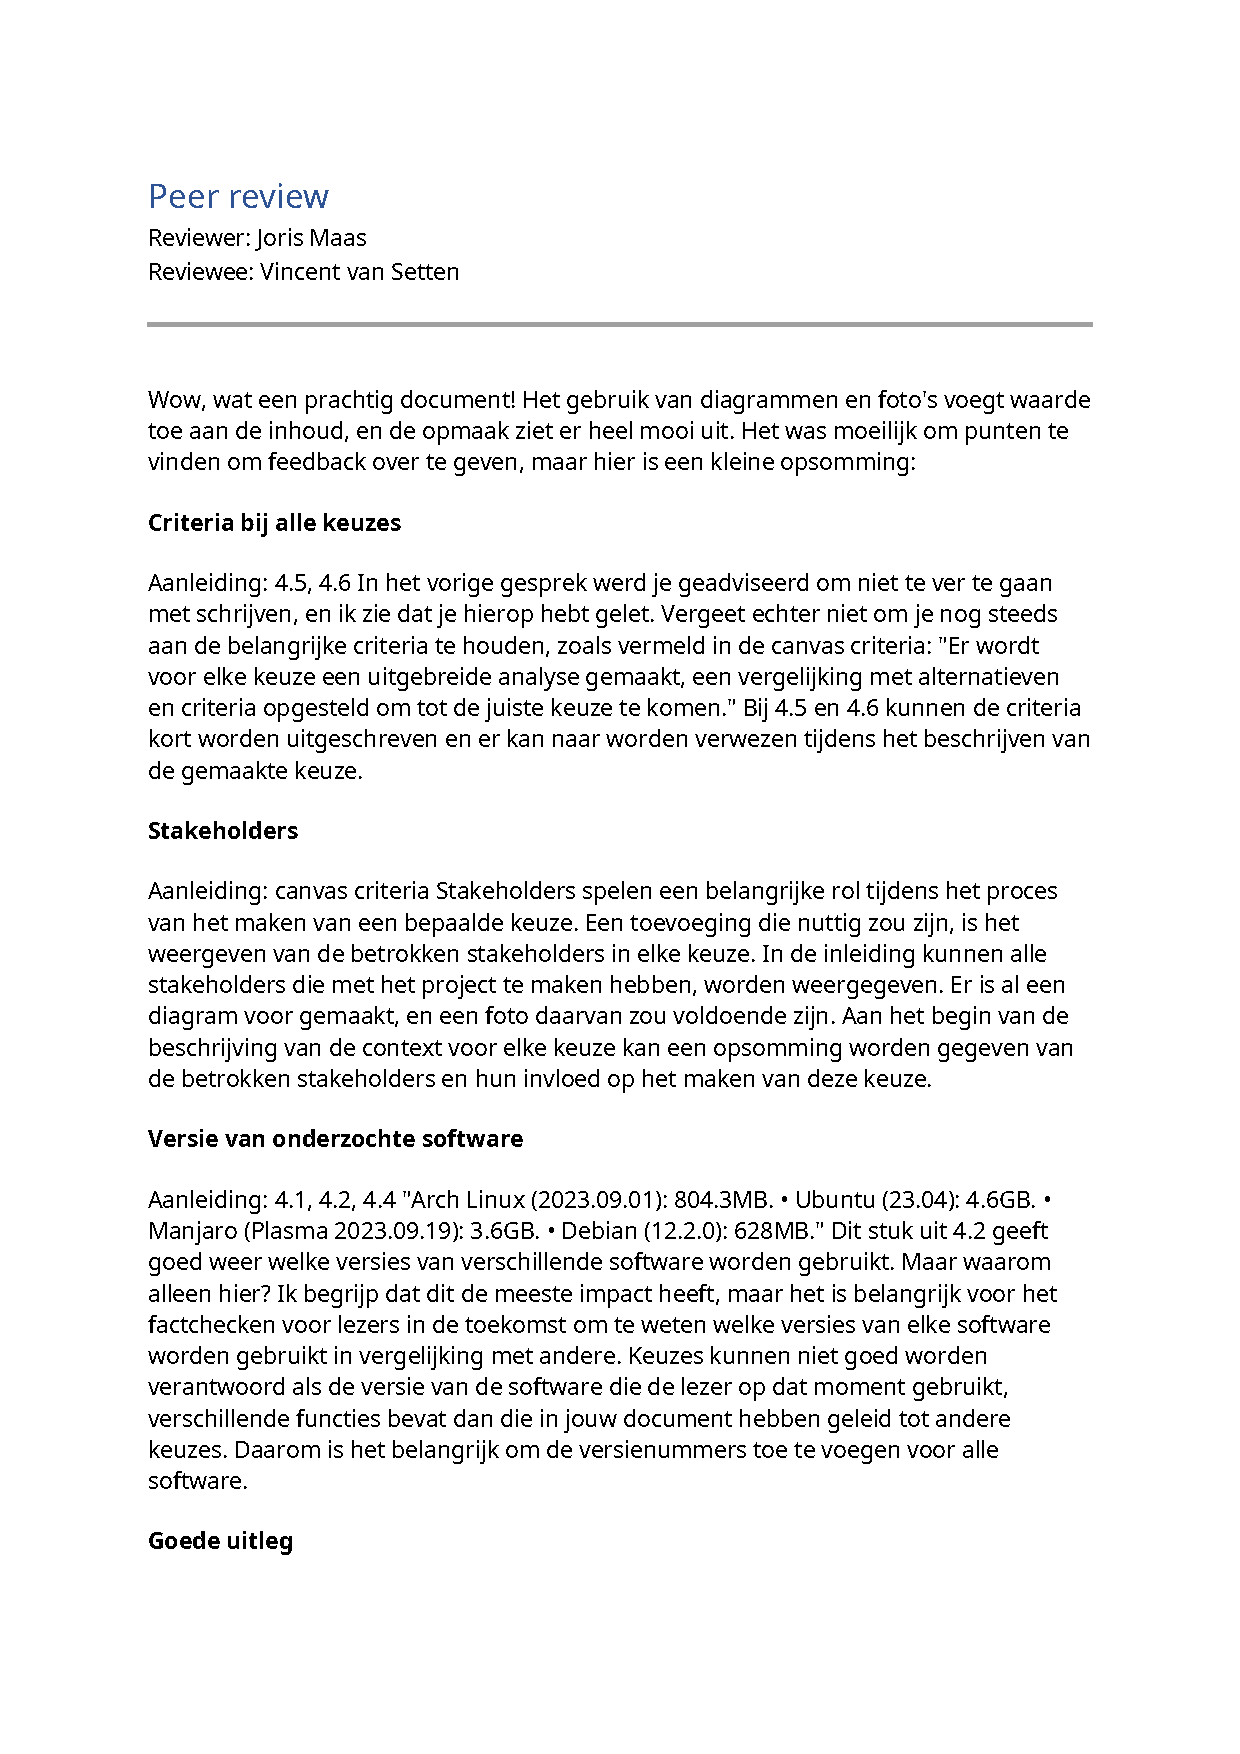
\includegraphics[page=1,scale=0.7]{Appendices/Iteratie 2/PR Vincent van Joris.pdf}}
\end{minipage}

\includepdf[pages={2},scale=0.7,frame,pagecommand={}]{Appendices/Iteratie 2/PR Vincent van Joris.pdf}

\subsection{Iteratie 3}
\subsubsection{Kyrill Westdorp}
\noindent
\begin{minipage}{\textwidth}
  \centering
  \fbox{
  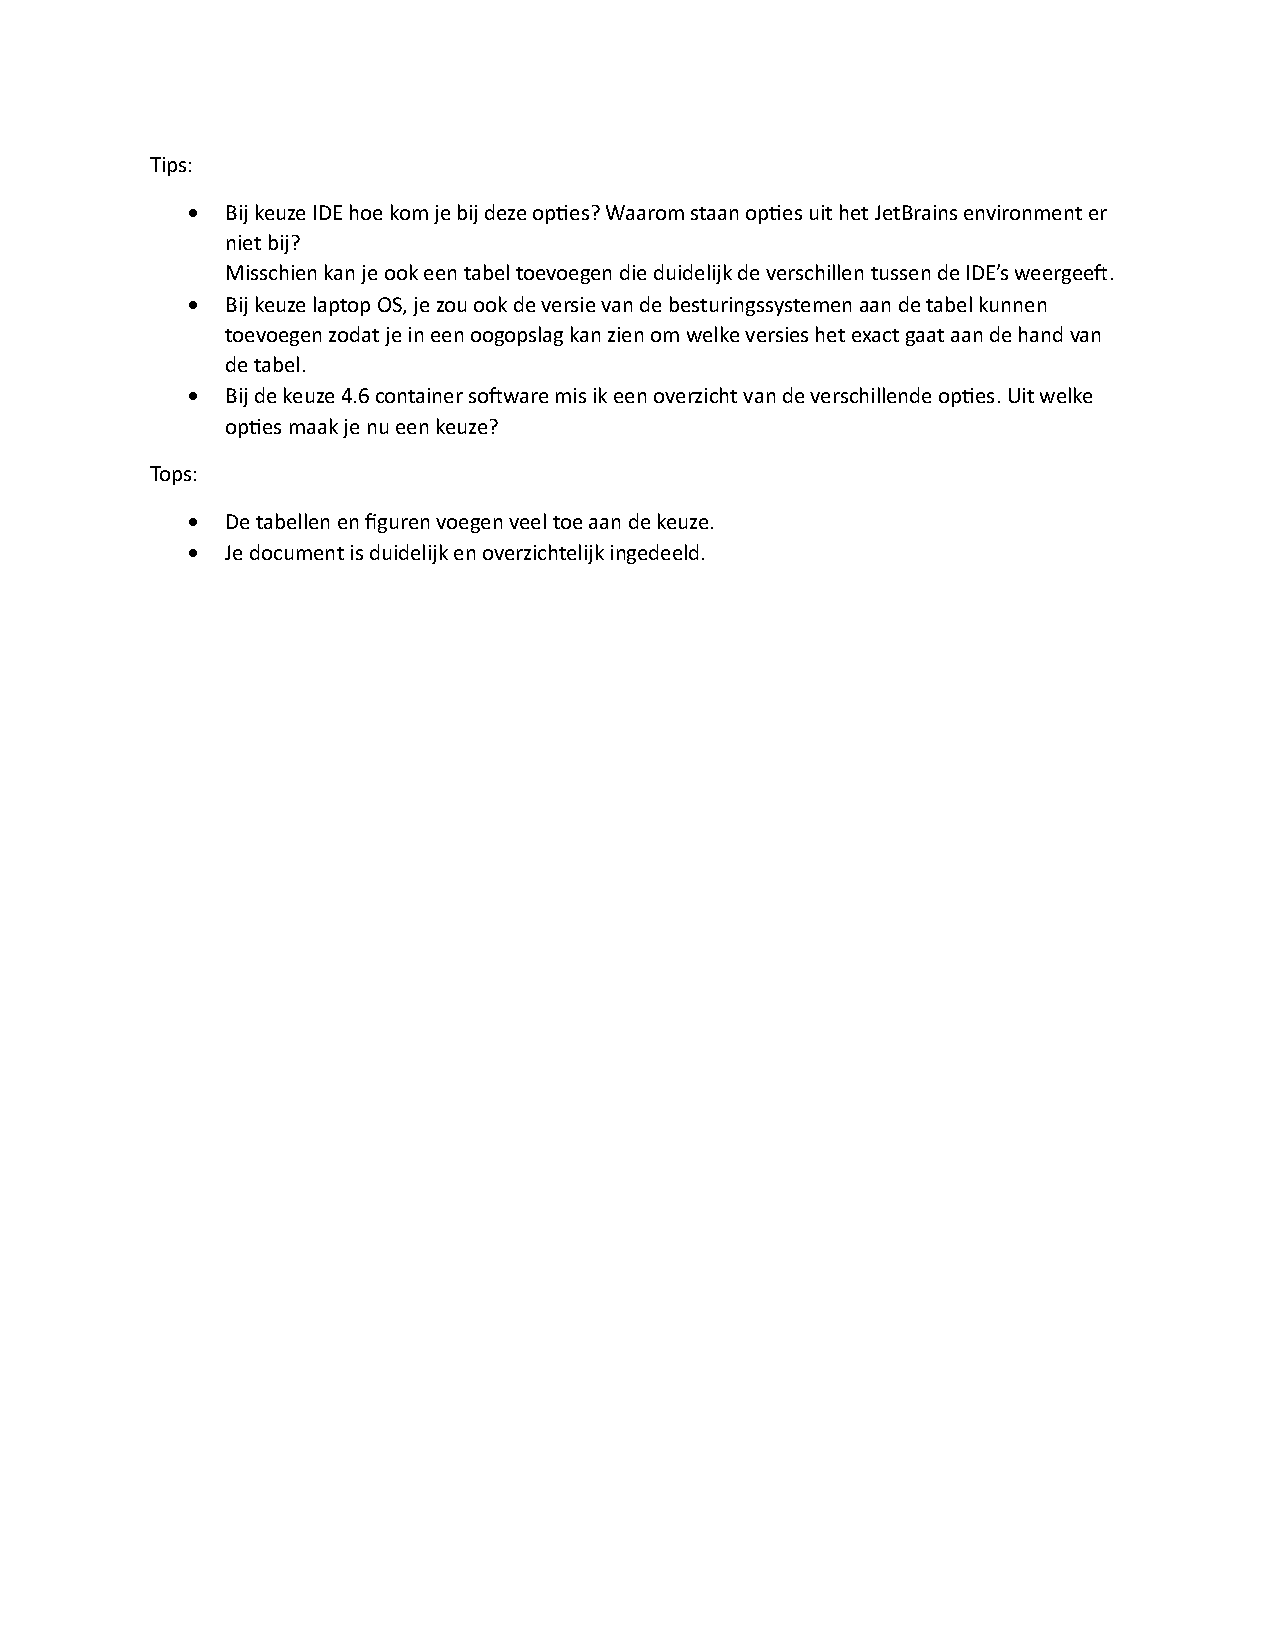
\includegraphics[page=1,scale=0.7]{Appendices/Iteratie 3/Review Vincent van Kyrill.pdf}}
\end{minipage}

\subsubsection{Jasper Middendorp}
\noindent
\begin{minipage}{\textwidth}
  \centering
  \fbox{
  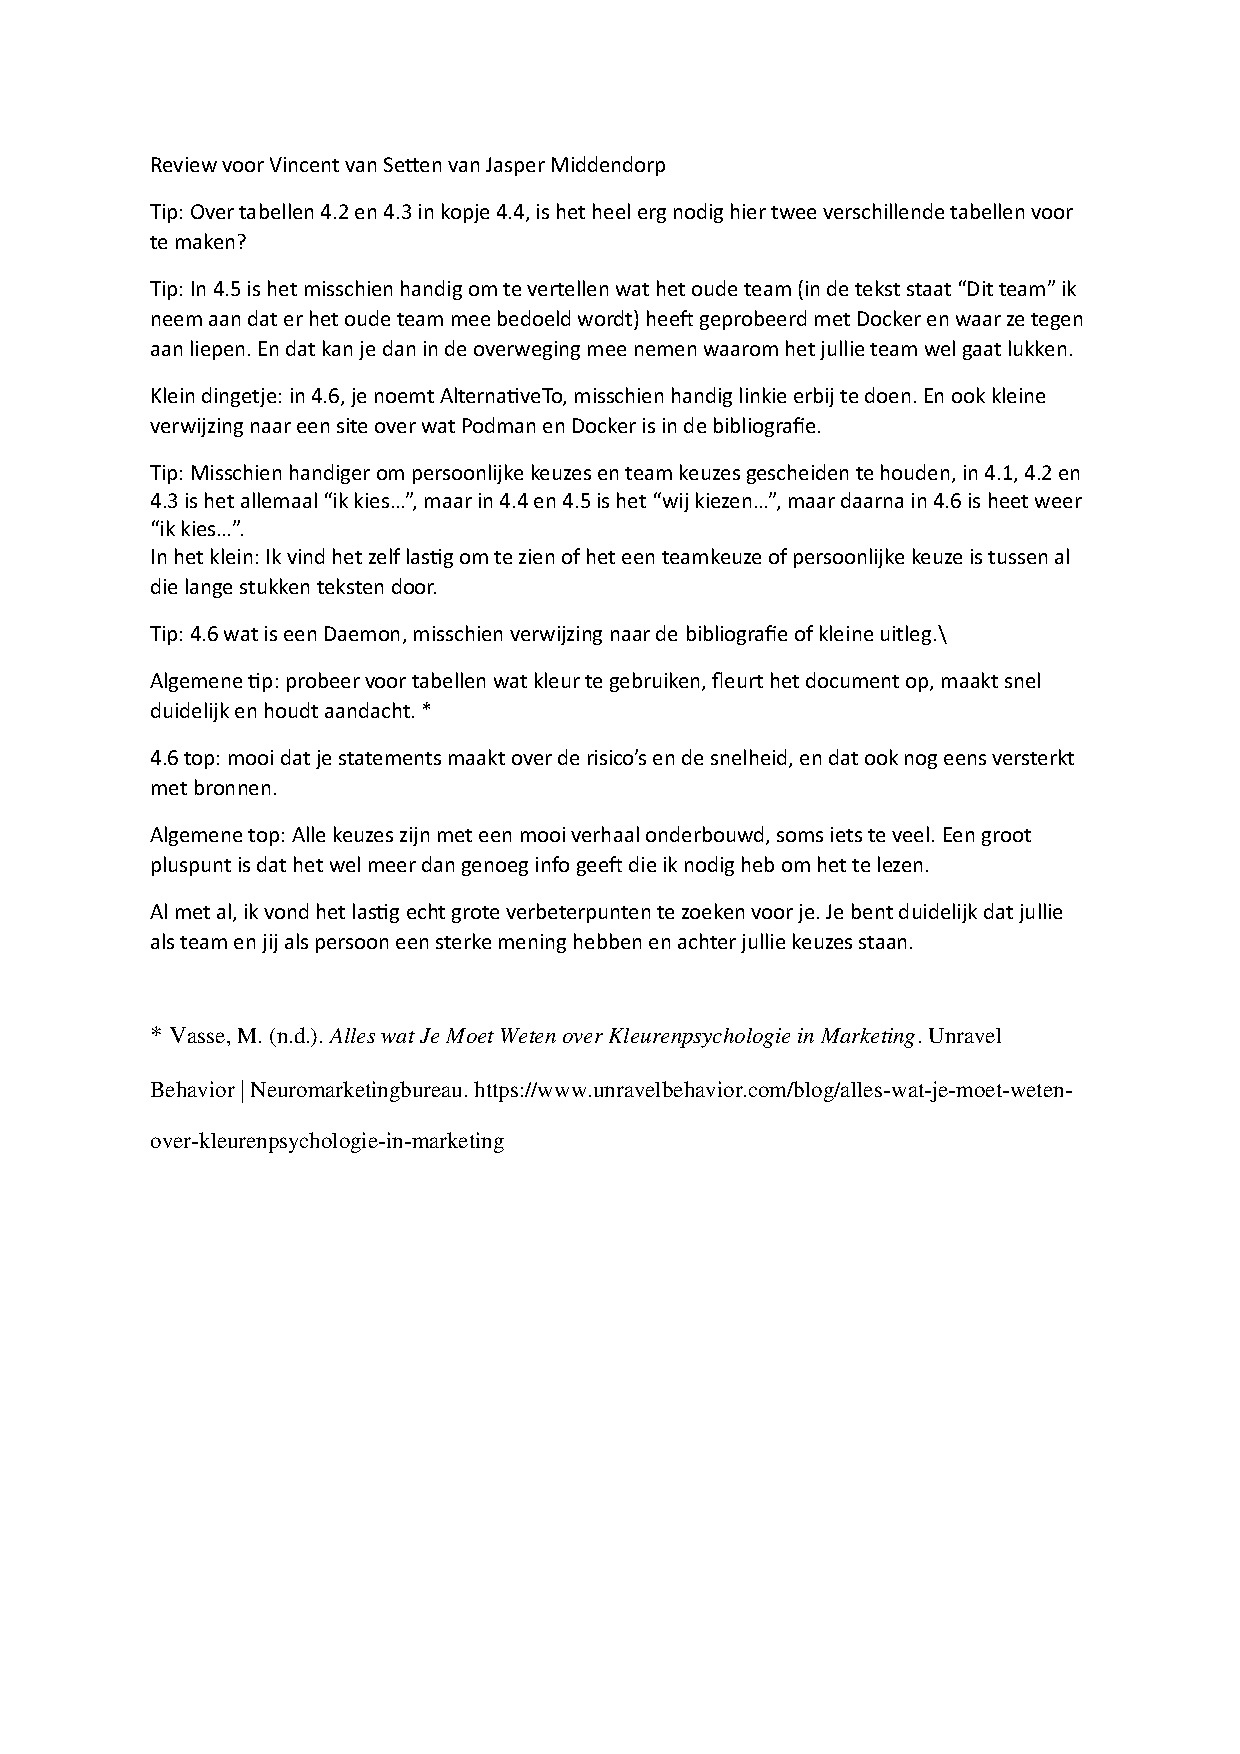
\includegraphics[page=1,scale=0.7]{Appendices/Iteratie 3/Review voor Vincent van Setten van Jasper Middendorp.pdf}}
\end{minipage}

\subsection{Iteratie 4}
\subsubsection{Joris Maas}
\noindent
\begin{minipage}{\textwidth}
  \centering
  \fbox{
  
\includegraphics[page=1,scale=0.7]{Appendices/Iteratie 4/PR Vincent van Joris.pdf}}
\end{minipage}
\clearpage

\subsubsection{Remy de Bruijn}
\noindent
Tips:
\begin{itemize}
  \item er kan nog iets beter uitgelegd worden waarom je tot de drie opties gekomen bent bij IDE gedeelte
  \item bij persoonlijke keuzes voor IDE vergelijk je drie opties, maar er is niet een duidelijke vergelijking te zien tussen de drie opties
  \item het enige wat mist bij 4.2 Laptop OS is een uitleg waarom je niet nog meer Linux distro's met elkaar vergelijkt dan de distro's die je hebt en waarom je je beperkt hebt tot dit aantal opties
  \item ik zag dat je feedback verwerkt had in je document van een vorige iteratie, maar de data bij de kopjes zijn niet aangepast om dat te reflecteren, dat maakt het moeilijk zoeken naar de feedback die je verwerkt hebt. Is gemakkelijk op te lossen door de datum aan te passen
\end{itemize}

Tops:
\begin{itemize}
  \item overzichtelijk document
  \item het lijkt ingekort of in ieder geval duidelijker
  \item goed feedback verwerkt van vorige keer
\end{itemize}


\pagebreak
\subsection{Verwerkte Feedback}
\subsubsection{Iteratie 3 feedback}
\label{verwerktefeedback1}
De volgende feedback heb ik verwerkt in iteratie 4 n.a.v. de ontvangen feedback van iteratie 3.
\begin{enumerate}
  \item Versie nummers van vergeleken OS's toegevoegd in de 'Laptop OS' keuze(4.2).
  \item Docker keuze(4.5) aangepast: de naam docker vervangen met 'Container (software)', omdat de keuze generieker was bedoeld.
  \item Definitie van 'Daemon' toegevoegd als footnote in hoofdstuk 4.6.
  \item Alle externe links duidelijk gemaakt in het gehele document(nu aangegeven met blauwe tekstkleur en een underline).
\end{enumerate}
\end{document}